\documentclass[../fractal_dimensions_quasicrystals.tex]{subfiles}
\begin{document}

\begin{figure}[htp]
\centering
    	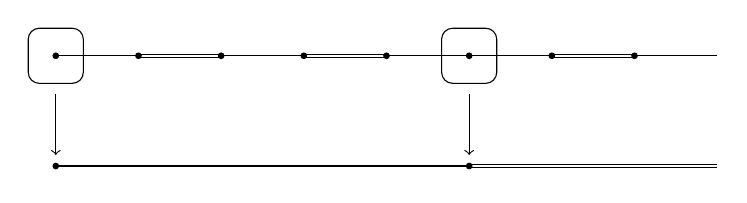
\begin{tikzpicture}[scale=.7]
    		\newcommand{\orig}{-1.5}
    		\newcommand{\trans}{1.5}
    		\newcommand{\vertspac}{-2.}
    		\newcommand{\vertsize}{.5} % vertical spand of the rectangles
    		\newcommand{\del}{.2}
    	
    		% initial chain
    	
    		% bonds 
        	\draw[-] (\orig, 0)  node [left] {}  -- (\orig+\trans, 0);
			\draw[-,double] (\orig+\trans,0) -- (\orig+2*\trans,0); % node [midway, above] {$t_s$};
			\draw[-] (\orig+2*\trans,0) -- (\orig+3*\trans,0); % node [midway, above] {$t_w$};	
			\draw[-,double] (\orig+3*\trans,0) -- (\orig+4*\trans,0); % node [midway, above] {$t_s$};
			\draw[-] (\orig+4*\trans,0) -- (\orig+5*\trans,0); % node [midway, above] {$t_w$};
			\draw[-] (\orig+5*\trans,0) -- (\orig+6*\trans,0); % node [midway, above] {$t_w$};
			\draw[-,double] (\orig+6*\trans,0) -- (\orig+7*\trans,0); % node [midway, above] {$t_s$};
			\draw[-] (\orig+7*\trans,0) -- (\orig+8*\trans,0); % node [midway, above] {$t_w$};
    	
    		% sites
			\foreach \x in {0,...,7}
		      \filldraw (\orig+\x*\trans,0) circle (0.05); % node [below] {$\ket{\x}$};
		      
		    % rectangles around atoms
		    \draw [rounded corners] (\orig-\vertsize,-\vertsize) rectangle (\orig+\vertsize,\vertsize);
		    \draw [rounded corners] (\orig-\vertsize+5*\trans,-\vertsize) rectangle (\orig+\vertsize+5*\trans,\vertsize);
		    
		    % arrows below rectangles
		    \draw [->] (\orig,-\vertsize-\del) -- (\orig,\vertspac+\del);
		    \draw [->] (\orig+5*\trans,-\vertsize-\del) -- (\orig+5*\trans,\vertspac+\del);
		      
		    % atomic chain
		    
        	\draw[-] (\orig, \vertspac)  node [left] {}  -- (\orig+5*\trans, \vertspac);
			\draw[-,double] (\orig+5*\trans,\vertspac) -- (\orig+8*\trans,\vertspac); % node [midway, above] {$t_s$};
			
			\filldraw (\orig,\vertspac) circle (0.05); % node [below] {$\ket{\x}$};
			\filldraw (\orig+5*\trans,\vertspac) circle (0.05); % node [below] {$\ket{\x}$};
%			\filldraw (\orig+8*\trans,\vertspac) circle (0.05); % node [below] {$\ket{\x}$};
		\end{tikzpicture}
\caption{The atomic deflation rule illustrated. Here we relate the fifth approximant to the second.}
\label{fig:at_defl}
\end{figure}

\end{document}